\documentclass{IOS-Book-Article}

\usepackage{mathptmx}
\usepackage{soul}
\setuldepth{article}
%\usepackage{times}
%\normalfont
%\usepackage[T1]{fontenc}
%\usepackage[mtplusscr,mtbold]{mathtime}
%
\def\hb{\hbox to 11.5 cm{}}

\usepackage{url}
\usepackage[colorlinks = true]{hyperref}
\usepackage[utf8]{inputenc}
%\usepackage[small]{caption}
\usepackage{graphicx}
\usepackage{amsmath,amsthm,amsfonts,amssymb}
\usepackage{subcaption}
\usepackage{booktabs}
\usepackage{xcolor}
%
\def\hb{\hbox to 11.5 cm{}}


\newtheorem{example}{Example}
\newtheorem{theorem}{Theorem}
\newtheorem{definition}{Definition}
\newtheorem{proposition}{Proposition}
\newtheorem{lemma}{Lemma}
\newcommand{\attrel}{\mathbf{R}}
\newcommand{\snake}{\mathrel\vert\mathrel{\mkern-3mu}\sim}
\newcommand{\nc}[2]{\snake^{#1}_{#2}}
%\newcommand{\nnc}[2]{\not\snake^{#1}_{#2}}
\newcommand{\nnc}[2]{\mathrel\diagup\mathrel{\mkern-20mu}\vert\mathrel{\mkern-8mu}\sim^{#1}_{#2}}
\newcommand{\args}{\mathbf{A}}
\newcommand{\inducedaf}[1]{F(#1)}



\begin{document}

\pagestyle{headings}
\def\thepage{}
\begin{frontmatter}              % The preamble begins here.


%\pretitle{Pretitle}
\title{Argumentation-based Causal Reasoning}

%\markboth{}{April 2026\hb}
%\subtitle{Subtitle}

\author{\fnms{Lars} \snm{Bengel}\thanks{Corresponding Author: Lars Bengel, \href{mailto:lars.bengel@fernuni-hagen.de}{lars.bengel@fernuni-hagen.de}}},
\author{\fnms{Oleksandr} \snm{Dzhychko}},
\author{\fnms{Myriam} \snm{Kasten}},
\author{\fnms{Kai} \snm{Sauerwald}},
\author{\fnms{Matthias} \snm{Thimm}}

%\runningauthor{L. Bengel et al.}
%\runningtitle{TODO}
\address{Artificial Intelligence Group, University of Hagen, Germany}


\end{frontmatter}
%\markboth{April 2022\hb}{April 2022\hb}
%\thispagestyle{empty}
%\pagestyle{empty}

\paragraph{Introduction.}
Argumentation-based approaches are well suited to provide human-understandable explanations in various domains.
One such domain is causal reasoning, which is a highly relevant topic in artificial intelligence research.
In the following, we present our web-based tool for argumentation-based causal reasoning.

\paragraph{Theoretical Background.}
Our tool is built on the argumentation-based causal reasoning framework developed by Bengel et al.~\cite{DBLP:conf/comma/BengelBRT22,DBLP:conf/ratio/BengelBRT24}, from which we briefly recall the core concepts.
We consider Pearl's causal models, but restrict our attention to Boolean-valued variables~\cite{pearl2000causality}.
A causal model is a triple $(U,V,K)$, where $U$ is a set of \emph{background} atoms, $V$ is a set of \emph{explainable} atoms, and $K$ a set of formulas called \emph{Boolean structural equations}.
Background atoms represent uncontrollable variables determined outside of the model.
Every explainable atom $v$ is functionally dependent on other atoms of the model.
This dependency is specified by exactly one Boolean structural equation of the form $v \leftrightarrow \phi$.
Intuitively, this represents the causal mechanism by which $v$ is determined by the other atoms in the model.
We then consider a \textit{causal knowledge base} $\Delta=(K, A)$ to consist of a causal model $K$ and a set of assumptions $A$ on the background atoms.

The argumentative aspect of this method relies on a characterisation of reasoning with maximal consistent subsets based on the notion of \emph{argumentation frameworks} (AFs)~\cite{DBLP:journals/ai/Dung95,DBLP:conf/ijcai/Cayrol95}.
%An AF is a pair $F = (\args, \attrel)$ where $\args$ is a set whose elements are called \emph{arguments} and where ${\attrel} \subseteq \args \times \args$ is called the \emph{attack relation}~\cite{DBLP:journals/ai/Dung95}.
We induce arguments from a causal knowledge base $\Delta=(K,A)$ as follows~\cite{DBLP:conf/ijcai/Cayrol95}.
An argument is a pair $(\Phi, \psi)$ where $\Phi \subseteq A$ is a minimal set of assumptions (called the \emph{premises} of the argument) that, together with $K$, consistently entails $\psi$ (called the \emph{conclusion} of the argument). 
One argument \emph{undercuts} another if the conclusion of the former is the negation of one premise of the latter.
The set of all arguments $\args$ induced by $\Delta$, together with undercut as the attack relation $\attrel$, forms the AF $(\args, \attrel)$ induced by $\Delta$.
A set of arguments $E\subseteq \args$ is called \emph{conflict-free} if for all $a,b \in E$ we have $(a,b)\notin\attrel$.
Furthermore, $E$ is called \emph{stable} if $E$ is conflict-free and for every $a \in \args \setminus E$ there is a $b \in E$ such that $(b,a)\in\attrel$.
It then holds that, given some set of literals $\Phi$ (observation) of the causal atoms, the knowledge base $\Delta$ entails some conclusion $\psi$, written as $\Phi \nc{}{\Delta} \psi$, if and only if the conclusion $\psi$ is contained in every stable extension of the induced AF.


\paragraph{System Description.}

We implemented a web-based \emph{causal knowledge base editor} which allows the graphical modelling of causal models and performing causal-reasoning based on the induced AF as outlined above.
The editor is available online\footnote{\url{https://causal-knowledge-base-editor.aig.fernuni-hagen.de}}
and includes examples as well as a user guide.
It provides an interface for creating causal models which can subsequently be evaluated.
For that, the user can define assumptions for the background atoms as well as the potential observations.
They will then be shown the valid conclusions, an explanation of the dependencies and can also view sequence-based explanations of the conclusion arguments~\cite{conf/kr/BengelT25}.
Notably, one can freely switch views between causal model and the induced AF, which displays the underlying structure of each induced causal argument.
Figure~\ref{fig:example} shows an exemplary causal model and the corresponding AF together with the information regarding the evaluation of the causal model.

The causal knowledge base editor has been implemented in JavaScript and the source code is available online\footnote{\url{https://github.com/aig-hagen/aig-causal-knowledge-base-editor}}.
The graphical representation and editor for causal models and AFs has been implemented via the \texttt{aig-graph-component}\footnote{\url{https://github.com/aig-hagen/aig_graph_component}}, which is an open-source web component for working with graph representations.
The causal reasoning as well as the construction of argumentation frameworks and their semantics are performed via \texttt{TweetyProject}~\cite{Thimm:2017a}, a comprehensive collection of Java libraries for logical aspects of artificial intelligence and knowledge representation.

\begin{figure}
    \centering
    \setlength{\fboxsep}{0pt}%
    \setlength{\fboxrule}{0.5pt}%
    \begin{minipage}{0.479\linewidth}
    \fbox{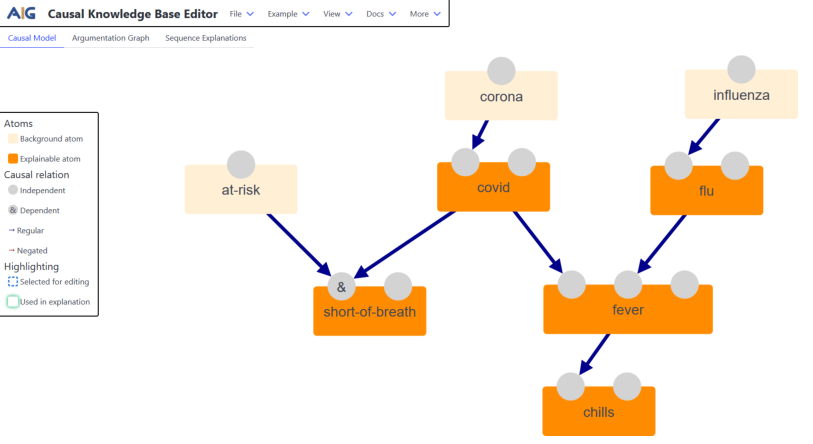
\includegraphics[width=0.975\linewidth]{figures/model.pdf}}
    \end{minipage}%
    \begin{minipage}{0.53\linewidth}
    
    \fbox{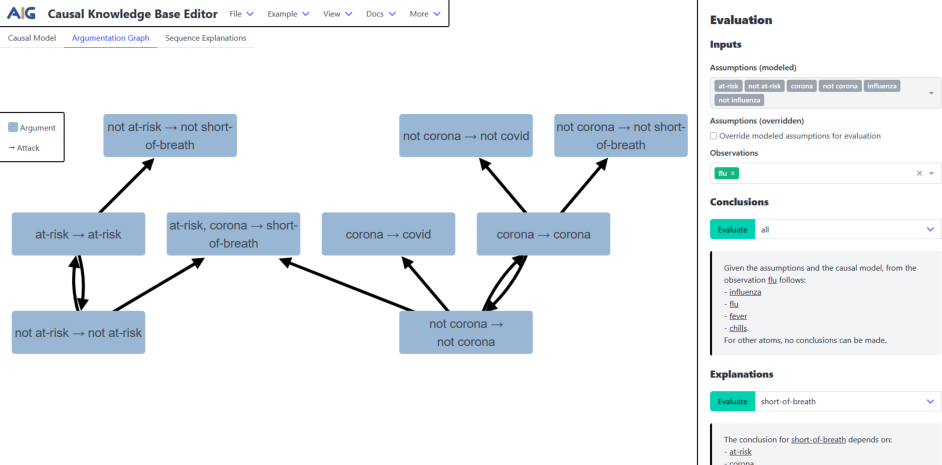
\includegraphics[width=0.975\linewidth]{figures/af.pdf}}
    \end{minipage}
    \caption{Screenshots of the editor showing an example causal model regarding the diagnosis of a viral disease (left) and the induced AF and its evaluation (right).}
    \label{fig:example}
\end{figure}



\paragraph{Future work.}
We intend to incorporate further ideas for presenting and explaining the results within the AF.
Furthermore, we plan to implement counterfactual reasoning via the twin model method as described in \cite{DBLP:conf/comma/BengelBRT22}.


\bibliographystyle{vancouver}
\bibliography{references.bib}

\end{document}
